\documentclass[indexstructuren.tex]{subfiles}
\begin{document}


\chapter{Theorie}
\section{Indexen}
\begin{de}
Een \textbf{index} is een toegangsstructuur dat ervoor hoort te zorgen dat de toegang tot een bestand word vergemakkelijkt.
\end{de}
\begin{de}
We noemen een bestand \textbf{ge\"indexeerd} op een gegeven attribuut als er een index voor bestaat om de toegang tot dat bestand te vergemakkelijken in verband met dat attribuut.
\end{de}

\section{Eigenschappen van indexen}
\begin{de}
Aantal records: $r$
\end{de}

\begin{de}
Aantal blokken: $b$
\[
b = \left\lceil \frac{r}{bfr} \right\rceil
\]
\end{de}

\begin{de}
De recordlengte: $R$
\end{de}

\begin{de}
De bloklengte: $B$
\end{de}

\begin{de}
Het aantal mogelijke unieke waarden voor een veld $w$: $u_w$.
\end{de}

\begin{de}
De \textbf{blocking factor} $bfr$ bepaalt hoeveel records er in \'e\'en block passen.
\[
bfr = \left\lfloor \frac{B}{R} \right\rfloor
\]
\end{de}
Omdat een index ook een bestand met records is kunnen we deze begrippen ook in de context van indexen gebruiken. We gebruiken dan een subscript $_i$.
Voor een dichte index geldt $r_i = r$, maar voor een index met ankerrecords geldt $r_i = b$.
\begin{de}
De blocking factor van een index wordt ook wel de \textbf{fan-out} $fo$ genoemd.
\[
bfr_i = fo
\]
\end{de}

\section{Enkelvoudige indexen (single-level indexes)}
\subsection{Primaire indexen (Primary indexes)}
Dit soort index houdt voor elk blok in de relatie een wijzer bij van het eerste record in het blok naar dat blok. Het eerste record in elk blok wordt een ankerrecord of een blokanker genoemd.

\subsubsection*{Voorwaarden}
\begin{itemize}
\item Veld dat ordening bepaald
\item Geordend data bestand
\item Index op veld met unieke waarden
\end{itemize}
\subsubsection*{Eigenschappen}
\begin{itemize}
\item
Er zijn precies zoveel records in de index als er blokken zijn in de relatie.
\[
r_i = b
\]
\end{itemize}

\subsection{Clusterende indexen (Clustering Indexes)}
Een clustering index is ook een index op een geordend veld, bij een geordend databestand. In een clusterende index bevat de index een wijzer van elke mogelijke waarde voor het veld naar de eerste  record dat die waarde heeft.

\subsubsection*{Voorwaarden}
\begin{itemize}
\item Veld dat ordening bepaald
\item Data bestand geordend op dat veld.
\item Klein aantal mogelijke waarden (veel kleiner dan het aantal records).
\end{itemize}
\subsubsection*{Eigenschappen}
\begin{itemize}
\item
Er zijn precies zoveel records in de index als er mogelijke waarden voor het veld.
\end{itemize}

\subsection{Secundaire indexen (Secondary Indexes)}
Een secundaire index biedt eenvoudigere toegang tot een bestand via een ander veld dan hetgeen waar het op geordend is.

\subsubsection{Secundaire index op een veld met unieke waarden}
In een secundaire index wordt voor elk record een wijzer bijgehouden naar dat record. Dit soort index is dens.\\
Er zijn precies zoveel records in de index als er records zijn in de relatie. Omdat een wijzer kleiner is dan een record is de blocking factor van de index groter dan de blocking factor van de relatie.
\[
r_i = r
\]
\[
R_i < R \Rightarrow bfr_i > bfr
\]
\subsubsection{Secundaire index op een ander veld}
In dit geval zijn er drie mogelijkheden
\begin{enumerate}
\item We houden duplicaten bij.
\item Voor elk duplicaat houden we de \emph{lijst} van wijzers bij naar de records.
\item Voor elk duplicaat houden we een extra niveau van indirectie bij.
\end{enumerate}

\subsection{Samenvatting}
\begin{figure}[H]
\centering
\begin{tabular}{c|c|c|}
& databestand geordend op indexveld & databestand niet geordend op indexveld\\\hline
veld met unieke waarden & Primaire index & Secundaire index(1)\\\hline
veld met niet-unieke waarden & Clusterende index & Secundaire index (2)\\\hline
\end{tabular}
\end{figure}
\begin{figure}[H]
\centering
\begin{tabular}{c|c|c|c}
Index type & Aantal indexrecords & Densiteit & Blok ankers\\\hline\hline
Primair & $b$ & spaars & ja\\
Clusterend & $u_{veld}$ & spaars & nee\\
Secundair (1) & $r$ & dens & nee\\
Secundair (2) & $u_{veld}$ & spaars & nee\\
\end{tabular}
\end{figure}

\section{Meervoudige indexen (multi-level indexes)}
Het idee achter meervoudige indexen is dat we het aantal indexblokken dat gelezen moet worden nog verkleind kan worden. Dit is beter dan binair zoeken omdat de blocking factor van de index$bfr_i$ groter is dan twee.
Omdat het eerste niveau van indexering een bestand is dat geordend is op een veld met unieke waarden, kunnen we hier een primaire indexering op maken met (ankerblokken).
Die indexering kunnen we opnieuw indexeren. 
Zo gaan we voort tot al de records van de bovenste indexering in \'e\'en blok passen. 

\noindent Het aantal niveaus van indexering vinden we dan als volgt.
\[
t = \lceil \log_{fo}(r_1) \rceil
\]

\section{B en B+ bomen}
Een B en B+ bomen zijn dynamische indexstructuren. het zijn gebalanceerde bomen van orde $p$. TODO

\newpage
\begin{figure}[H]
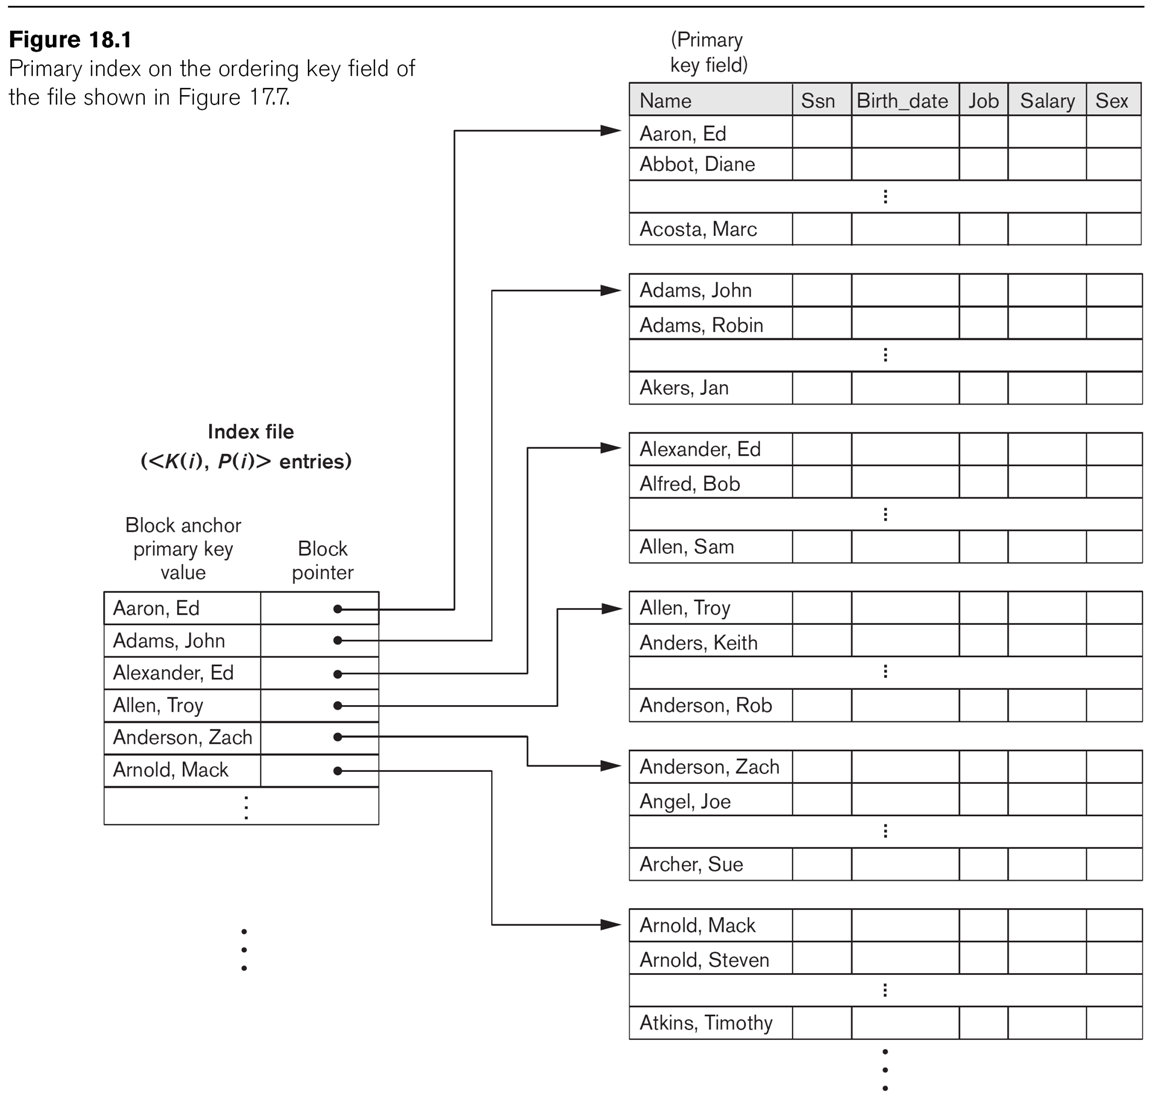
\includegraphics[width=\linewidth]{illustraties/primaire_index.png}
\caption{Primaire index}
\end{figure}
\begin{figure}[H]
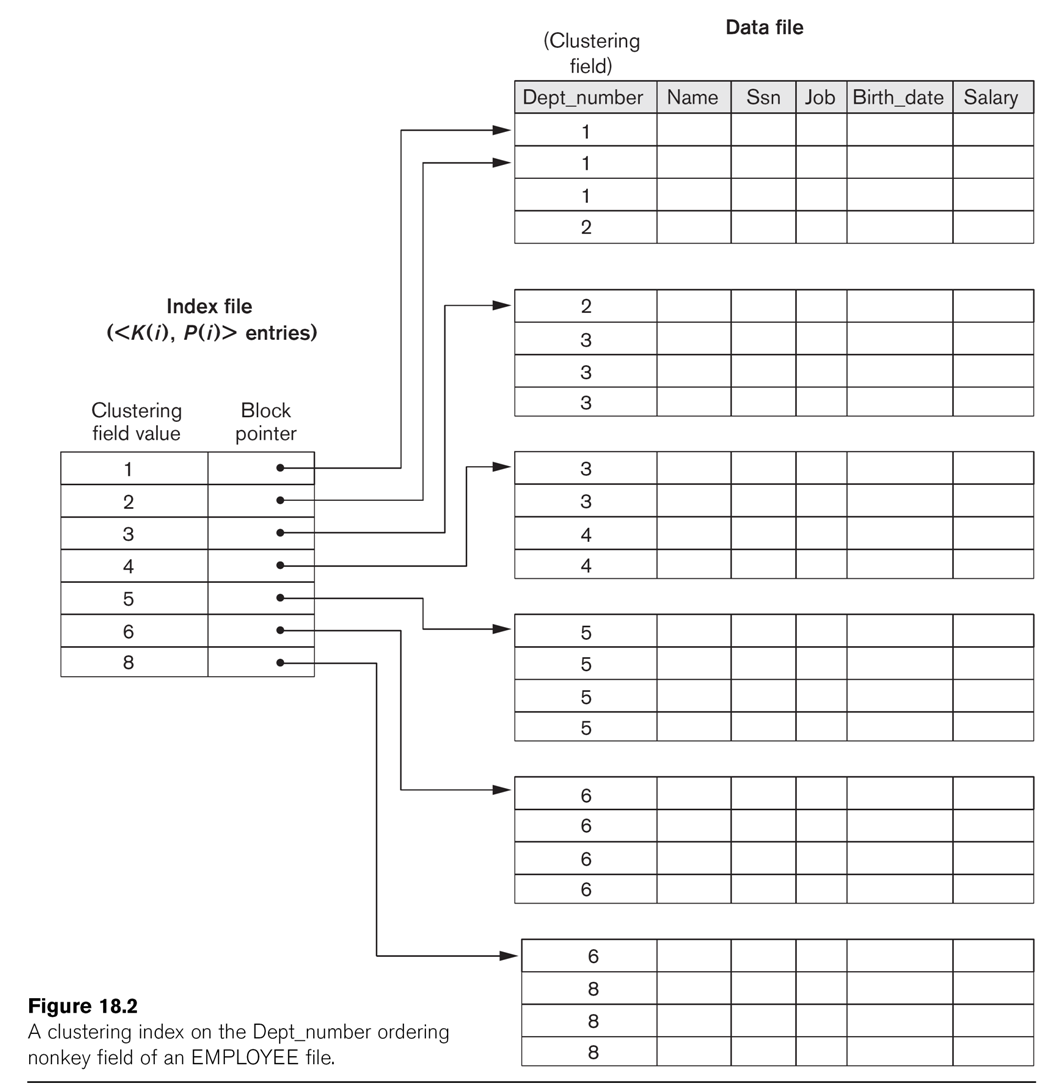
\includegraphics[width=\linewidth]{illustraties/clustering_index.png}
\caption{Clusterende index}
\end{figure}
\begin{figure}[H]
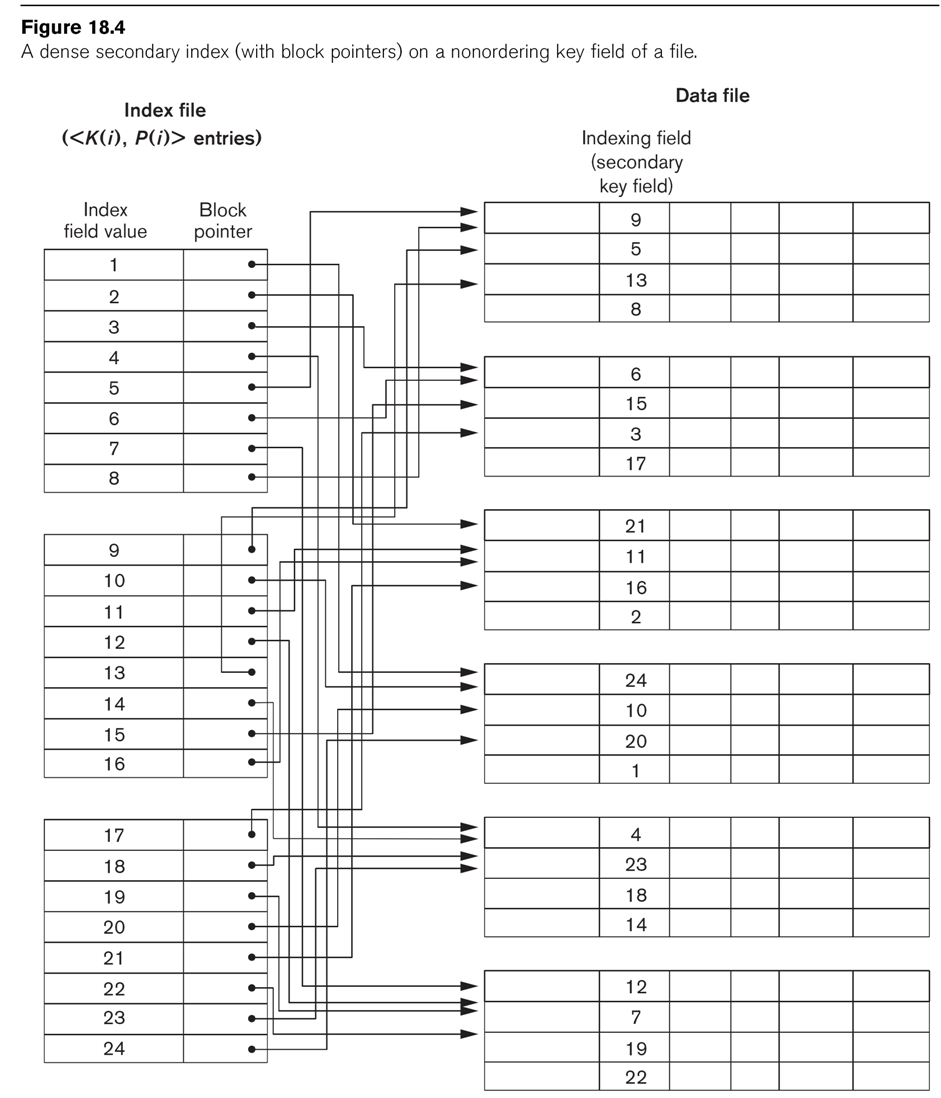
\includegraphics[width=\linewidth]{illustraties/secondaire_index.png}
\caption{Secundaire index (1)}
\end{figure}
\begin{figure}[H]
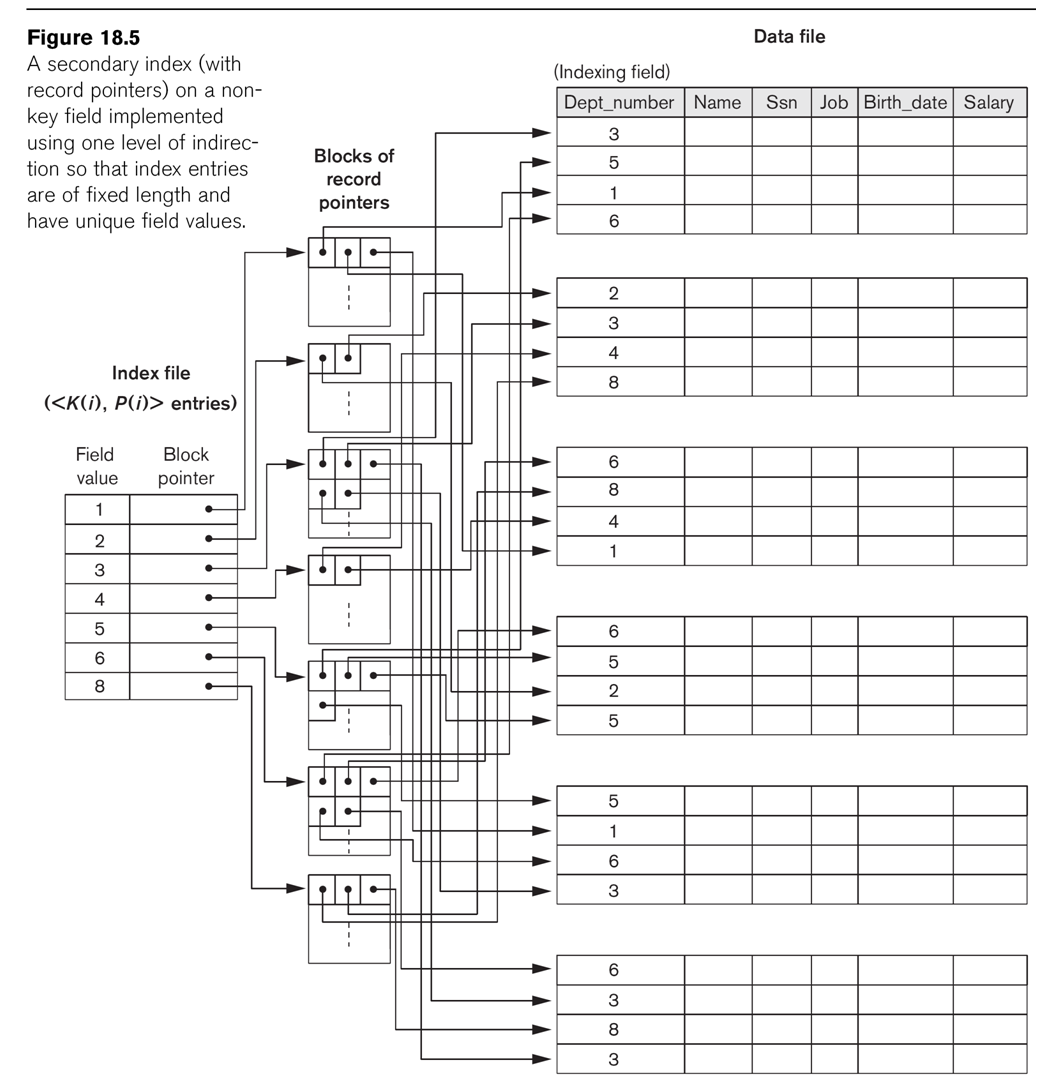
\includegraphics[width=\linewidth]{illustraties/secondaire_index2.png}
\caption{Secundaire index (2)}
\end{figure}
\begin{figure}[H]
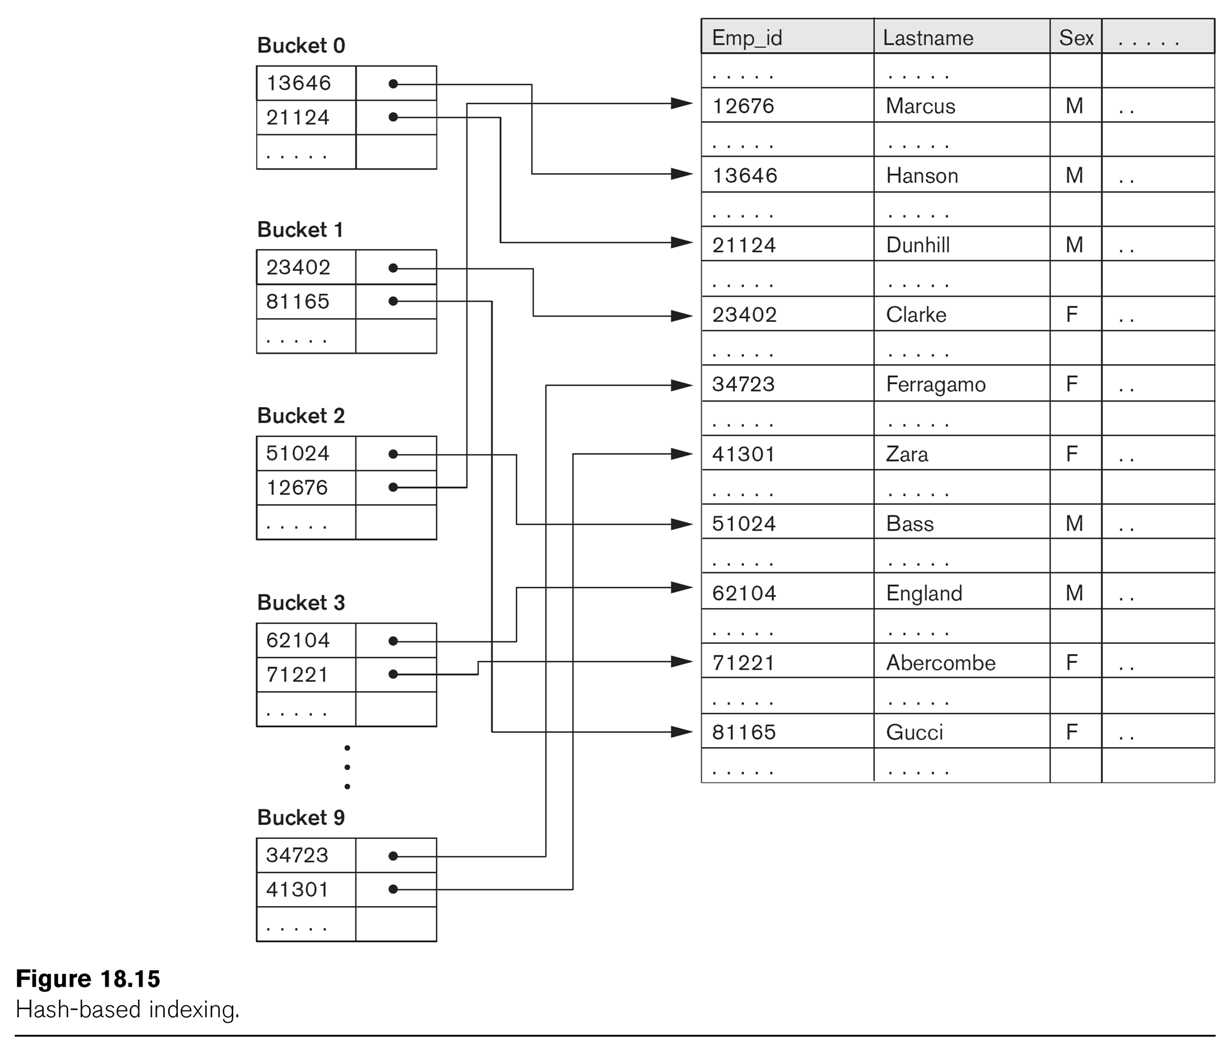
\includegraphics[width=\linewidth]{illustraties/hash_index.png}
\caption{Hash index}
\end{figure}
\begin{figure}[H]
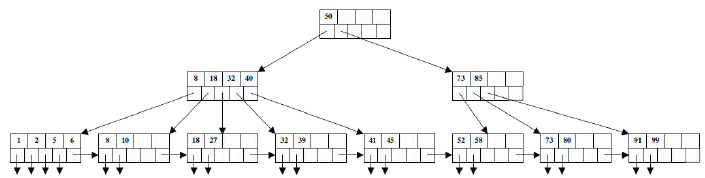
\includegraphics[width=\linewidth]{illustraties/b_plus_tree.png}
\caption{B+ boom}
\end{figure}

\end{document}
